\PassOptionsToPackage{unicode=true}{hyperref} % options for packages loaded elsewhere
\PassOptionsToPackage{hyphens}{url}
%
\documentclass[12pt,]{article}
\usepackage{lmodern}
\usepackage{amssymb,amsmath}
\usepackage{ifxetex,ifluatex}
\usepackage{fixltx2e} % provides \textsubscript
\ifnum 0\ifxetex 1\fi\ifluatex 1\fi=0 % if pdftex
  \usepackage[T1]{fontenc}
  \usepackage[utf8]{inputenc}
  \usepackage{textcomp} % provides euro and other symbols
\else % if luatex or xelatex
  \usepackage{unicode-math}
  \defaultfontfeatures{Ligatures=TeX,Scale=MatchLowercase}
\fi
% use upquote if available, for straight quotes in verbatim environments
\IfFileExists{upquote.sty}{\usepackage{upquote}}{}
% use microtype if available
\IfFileExists{microtype.sty}{%
\usepackage[]{microtype}
\UseMicrotypeSet[protrusion]{basicmath} % disable protrusion for tt fonts
}{}
\IfFileExists{parskip.sty}{%
\usepackage{parskip}
}{% else
\setlength{\parindent}{0pt}
\setlength{\parskip}{6pt plus 2pt minus 1pt}
}
\usepackage{hyperref}
\hypersetup{
            pdftitle={Mortalidad en áreas pequeñas de la región Pampeana (Argentina, 2009-2011)},
            pdfborder={0 0 0},
            breaklinks=true}
\urlstyle{same}  % don't use monospace font for urls
\usepackage[margin=1in]{geometry}
\usepackage{graphicx,grffile}
\makeatletter
\def\maxwidth{\ifdim\Gin@nat@width>\linewidth\linewidth\else\Gin@nat@width\fi}
\def\maxheight{\ifdim\Gin@nat@height>\textheight\textheight\else\Gin@nat@height\fi}
\makeatother
% Scale images if necessary, so that they will not overflow the page
% margins by default, and it is still possible to overwrite the defaults
% using explicit options in \includegraphics[width, height, ...]{}
\setkeys{Gin}{width=\maxwidth,height=\maxheight,keepaspectratio}
\setlength{\emergencystretch}{3em}  % prevent overfull lines
\providecommand{\tightlist}{%
  \setlength{\itemsep}{0pt}\setlength{\parskip}{0pt}}
\setcounter{secnumdepth}{0}
% Redefines (sub)paragraphs to behave more like sections
\ifx\paragraph\undefined\else
\let\oldparagraph\paragraph
\renewcommand{\paragraph}[1]{\oldparagraph{#1}\mbox{}}
\fi
\ifx\subparagraph\undefined\else
\let\oldsubparagraph\subparagraph
\renewcommand{\subparagraph}[1]{\oldsubparagraph{#1}\mbox{}}
\fi

% set default figure placement to htbp
\makeatletter
\def\fps@figure{htbp}
\makeatother

\usepackage{booktabs}
\usepackage{longtable}
\usepackage{array}
\usepackage{multirow}
\usepackage{wrapfig}
\usepackage{float}
\usepackage{colortbl}
\usepackage{pdflscape}
\usepackage{tabu}
\usepackage{threeparttable}
\usepackage{threeparttablex}
\usepackage[normalem]{ulem}
\usepackage{makecell}
\usepackage{xcolor}

\title{Mortalidad en áreas pequeñas de la región Pampeana (Argentina,
2009-2011)}
\author{Nicolás Sacco;\footnote{Penn State,
  \href{mailto:nsacco@psu.edu}{\nolinkurl{nsacco@psu.edu}}} Iván
Williams;\footnote{Universidad Nacional de Luján,
  \href{mailto:ivanwilliams1985@gmail.com}{\nolinkurl{ivanwilliams1985@gmail.com}}}
Bernardo L. Queiroz\footnote{Cedeplar-UFMG,
  \href{mailto:lanza@cedeplar.ufmg.br}{\nolinkurl{lanza@cedeplar.ufmg.br}}}}
\date{Agosto, 2019}

\begin{document}
\maketitle

\hypertarget{abstract}{%
\section{\texorpdfstring{\textbf{Abstract}}{Abstract}}\label{abstract}}

\hypertarget{background}{%
\subsection{\texorpdfstring{\textbf{Background}}{Background}}\label{background}}

Mientras aumenta la demanada sobre estimaciones epidemiológicas para
áreas pequeñas, estudios recientes muestran una persistente brecha de
desigualdad en la esperanza de vida al nacer en América Latina. La
escasez de datos geoespaciales desafía la aplicación de diferentes
métodos para estudiar estos diferenciales de salud. A menudo, los datos
en áreas pequeñas o bien no existen o son escasos en la región. Los
patrones espaciales son esenciales para comprender los resultados
demográficos individuales relacionados con las características de un
lugar, también como una herramienta para la aplicación de planes de
desarrollo y para la asignación de recursos.

\hypertarget{objectives}{%
\subsection{\texorpdfstring{\textbf{Objectives}}{Objectives}}\label{objectives}}

La historia de la estimación en áreas pequeñas es escasa en Argentina,
un claro ejemplo de un país con pocas fuentes de datos, pero también un
caso muy interesante de la transición epidemiológica, que a menudo no se
aborda en la literatura previa Basado en la experiencia de nuevas
aplicaciones y de acuerdo con la información auxiliar disponible, en
este artículo aplicamos tres métodos diferentes para estimar y luego
comparar los niveles de mortalidad en áreas pequeñas en la Región
Pampeana de Argentina, durante el período 2009-2011.

\hypertarget{methods}{%
\subsection{\texorpdfstring{\textbf{Methods}}{Methods}}\label{methods}}

Se calculó la esperanza de vida al nacer en base a un enfoque bayesiano,
un método de tabla de vida relacional, suavizando datos espaciales de
acuerdo a patrones de áreas mayores vecinas, y en tercer lugar se aplicó
un enfoque demográfico indirecto. Las estimaciones se compararon para
calcular las tasas de \(q_0\) a partir de registros de defunción
completos y luego se relacionaron con áreas espaciales, utilizando un
análisis de regionalización simple.

\hypertarget{results}{%
\subsection{\texorpdfstring{\textbf{Results}}{Results}}\label{results}}

Los resultados muestran el valor potencial del método bayesiano a
pequeña escala espacial-espacial. Las tasas estimadas indican que existe
una gran variabilidad en la esperanza de vida al nacer y entre regiones,
con una extensión de más de 6 años en la Provincia de Buenos Aires.
Además, encontramos evidencia sugestiva de que las tasas por edad
presentan una mayor mortalidad infantil, pero también un mayor riesgo en
los adultos mayores, en las provincias que muestran más heterogeneidad.

\begin{center}\rule{0.5\linewidth}{0.5pt}\end{center}

\hypertarget{introduction}{%
\subsection{\texorpdfstring{\textbf{Introduction}}{Introduction}}\label{introduction}}

¿Subsisten las disparidades de mortalidad entre las áreas pequeñas?
Investigaciones demográficas previas sobre los diferenciales de
mortalidad sostienen que los diferenciales geográficos serían
gradualmente descartados durante la transición epidemiológica, las
políticas de salud pública y las mejoras en la calidad de vida. En la
mayoría de los países de ingresos altos y medios, la esperanza de vida
al nacer (\(q_0\)) aumenta a principios del siglo XX, debido al avance
del conocimiento y la tecnología médica para combatir las enfermedades
infecciosas y las mejoras en las condiciones de vida asociadas con el
desarrollo socioeconómico.

Aunque los diferenciales socioeconómicos de mortalidad contribuyeron a
mantener la hipotesis de la desigualdad persistente en la muerte durante
y después de la transición epidemiológica, algunos autores esperan que
los resultados de salud y las disparidades se extingan a medida que se
desarrolla el cambio demográfico. Sin embargo, puntos de vista
retrospectivos muestran que los diferenciales de mortalidad son
persistentes y han crecido con el tiempo en muchos casos de acuerdo a la
condición socioeconómica. De todos modos, es útil tener en cuenta si
estas disparidades continúan y/o surgen independientemente de escenarios
iniciales auspiciosos.

La explicación teórica más persuasiva de estos temas argumenta que la
relación entre mortalidad y posición socioeconómica se ha mantenido a lo
largo del tiempo debido al acceso diferencial de clase social a la
tecnología de la información y a la salud. Esta hipótesis de
causa-efecto condujo a importantes desarrollos de investigación y
contribuciones teóricas. Sin embargo, identificar las relaciones basadas
en estos patrones y sus resultados demográficos presenta un serio
desafío en países donde hay pocas fuentes de datos disponibles. La
investigación de la mortalidad implica intrincadas patuas de
interacciones sociales, demográficas y ambientales. Por esa razón, la
demografía espacial surgió como una perspectiva significativa para
responder preguntas demográficas (Matthews, 2013). En ese sentido, los
patrones espaciales son esenciales para comprender los resultados
demográficos individuales relacionados con las características de un
lugar.

Sobre estas cuestiones, aportes metodológicas recientes se han
desarrollado para estimaciones de mortalidad en áreas pequeñas.
\textbf{\emph{Mas sobre aportes recientes para estimacion de mortalidad
en areas menores en el mundo.}}.

En América Latina y el Caribe, la demanda de estimaciones
epidemiológicas (y de mortalidad, específicamente) de la heterogeneidad
subnacional está creciendo, tanto como una herramienta para la
aplicación de diferentes planes de desarrollo como para la asignación de
recursos. La experiencia en América Latina está liderada por Brasil,
donde ya existe un desarrollo metodológico sostenido Freire
(\protect\hyperlink{ref-FreireEtAl2015}{2015}). En Argentina, se
encontraron experiencias sobre estimaciones de la tendencia de
mortalidad infantil (Torcida, Vega, and Velázquez
(\protect\hyperlink{ref-torcida2008}{2008})) y las comunas de la Ciudad
Autónoma de Buenos Aires (Grushka
(\protect\hyperlink{ref-Grushka2013}{2013})). Al mismo tiempo, otros
estudios se centran en el desarrollo de herramientas demográficas para
medir la heterogeneidad individual en una población (Vaupel and Missov
(\protect\hyperlink{ref-Vaupel_Missov_2013}{2013}); Raalte, Sasson, and
Martikainen
(\protect\hyperlink{ref-vanRaalte_Sasson_Martikainen_2018}{2018})). En
este sentido, solo considerando la información de la tabla de vida,
podría haber múltiples capas de análisis de desigualdad simplemente
agrupando por niveles administrativos.

Argentina representa un claro ejemplo de un país con pocas fuentes de
datos, pero también un caso muy interesante de la transición de la
mortalidad, que a menudo no se aborda en la literatura previa. Por estas
razones, el objetivo de este artículo fue el de elaborar estimaciones de
mortalidad que ejemplifiquen la relación entre el condición
socioeconómica y salud. Para ello aplicamos tres métodos diferentes para
estimar y luego comparar los niveles de mortalidad en áreas pequeñas en
la Región Pampeana Argentina, durante el período 2009-2011. Para probar
cómo funcionan los métodos elegidos, discriminamos este espacio
geográfico ya que es la región más poblada del país.

Debido a la poca experiencia de estudios previos que estimen mortalidad
\emph{general} en áreas menores en Argentina, se decidió aplicar tres
técnicas: una basada en la teoría bayesiana, la segunda basada en
métodos relacionales de tablas de vida pero agregando técnicas
estadísticas de suavizado, y tercero, un enfoque demográfico clásico,
considerado el método por default debido a su simplicidad. Antes de la
estimación, se realizó un procedimiento de regionalización para
aprovechar la similitud espacial entre áreas pequeñas,
independientemente de su pertenencia político-administrativa.

Utilizamos los datos administrativos del registro de defunciones del
Departamento de Estadísticas e Información de Salud del Ministerio de
Salud de la Nación (DEIS), unidad oficial del gobierno a cargo de la
administración de conteos de defunciones, y las estimaciones de
población elaboradas por el Instituto Nacional de Estadísticas y censo
(INDEC) agencia gubernamental argentina responsable de la recopilación y
el procesamiento de datos estadísticos, como los censos de población.
Usando tres enfoques diferentes, primero aplicamos Métodos de
Distribución de Muerte (DDM, por su sigla en inglés). Luego combinamos
DDM con un enfoque empírico bayesiano, método ya aplicado para el caso
de Brasil. El procedimiento de dos pasos nos permite corregir la falta
de registro de los recuentos de muertes y minimizar las fluctuaciones
aleatorias que pueden ocurrir cuando calculamos los niveles de
mortalidad en áreas pequeñas.

\hypertarget{por-quuxe9-argetinapor-quuxe9-la-regiuxf3n-pampeana}{%
\section{¿Por qué Argetina?¿Por qué la región
Pampeana?}\label{por-quuxe9-argetinapor-quuxe9-la-regiuxf3n-pampeana}}

En Argentina, se encontraron experiencias sobre estimaciones de la
tendencia de mortalidad infantil (Torcida, Vega, and Velázquez
(\protect\hyperlink{ref-torcida2008}{2008})) y las comunas de la Ciudad
Autónoma de Buenos Aires (Grushka
(\protect\hyperlink{ref-Grushka2013}{2013})). Al mismo tiempo, otros
estudios se centraron en el desarrollo de herramientas demográficas para
medir la heterogeneidad de mortalidad en una población (Vaupel and
Missov (\protect\hyperlink{ref-Vaupel_Missov_2013}{2013}); Raalte,
Sasson, and Martikainen
(\protect\hyperlink{ref-vanRaalte_Sasson_Martikainen_2018}{2018})). En
este sentido, solo considerando la información de la tabla de vida,
podría haber múltiples capas de análisis de desigualdad teniendo en
cuenta distintos niveles espaciales.

Este trabajo como fin tiene estimar el nivel de mortalidad para áreas
menores de Argentina, en este caso, de departamentos durante el período
2009-2011. Con el criterio de comenzar con la población con mayor
participación en total país se seleccionó la región pampeana.

Se propone la siguiente línea de desarrollo. Se realiza un análisis
inicial de calidad de datos, se repasan tres metodologías de
suavizamiento, redefiniendo a su vez áreas mayores por fuera de lo
estrictamente administrativo, se construyen tablas de mortalidad y se
selecciona un método con el cual dar una primera aproximación al
problema. En el medio se encuentraron inconvenientes con la información,
los cuales se trataron de destacar y dar soluciones\footnote{El material
  complementario, código y resultados se pueden encontrar en
  \url{https://github.com/nsacco/mortalidad_Argentina}.}.

Este trabajo como fin tiene estimar el nivel de mortalidad para áreas
menores de Argentina, en este caso, de departamentos durante el período
2009-2011. Con el criterio de comenzar con la población con mayor
participación en total país se seleccionó la región pampeana.

The lack of geospatial data challenge the application of different
methods to study health differentials. Often data in small areas are
non-existent or sparce in this region. Spatial patterns are essential to
understand individual demographic outcomes related with the
characteristics of a place, also as a tool for the application of
development plans and for the allocation of resources.

En América Latina y el Caribe, la demanda de estimaciones
epidemiológicas (y de mortalidad, específicamente) sobre heterogeneidad
a nivel subnacional está creciendo, tanto como una herramienta para la
aplicación de diferentes planes de desarrollo como para la asignación de
recursos. La pregunta es siempre: ¿qué esconden los promedios
regionales?

El problema principal es el de tratar con fenómenos con un pequeño
número de experimentos, y en muchos casos desconocida cobertura. La
experiencia en América Latina está liderada por Brasil, donde ya existe
un desarrollo metodológico de avance sostenido (Freire
(\protect\hyperlink{ref-FreireEtAl2015}{2015})).

En América Latina y el Caribe, la demanda de estimaciones
epidemiológicas (y de mortalidad, específicamente) sobre heterogeneidad
a nivel subnacional está creciendo, tanto como una herramienta para la
aplicación de diferentes planes de desarrollo como para la asignación de
recursos. La pregunta es siempre: ¿qué esconden los promedios
regionales?

The objective of this work can be enunciated following these progressive
steps:\\
+ Estimate the level of mortality of the departments during the period
2009-2011. With the criteria of starting with the population with bigger
share to explore methodological approaches, the Pampean region was
selected.\\
+ Estimate the heterogeneity between and within departments.\\
+ Test the hypothesis of the negative relationship between internal
heterogeneity and the level of mortality at the province level.

In this first work, the step 1 is done.\footnote{All the supplemental
  material, code and results can be found in
  \url{https://github.com/nsacco/mortalidad_Argentina}. It´s work in
  progress}

El problema principal es el de tratar con fenómenos con un pequeño
número de experimentos, y en muchos casos desconocida cobertura. La
experiencia en América Latina está liderada por Brasil, donde ya existe
un desarrollo metodológico de avance sostenido (Freire
(\protect\hyperlink{ref-FreireEtAl2015}{2015})).

In comparison with other Latin American countries, Argentina's early
socio-economic development, high degree of urbanization, and the
expansion of formal education all influenced the reduction of mortality
taking place earlier than in most other countries of the region. This
took place due to improvements in living conditions associated with
socioeconomic development, rather than the advancement of knowledge and
medical technology to fight infectious diseases. Although it took place
more quickly and began from higher levels, the drop in mortality in
Argentina can, in that sense, be likened to the pattern followed by
developed countries with greater distance then from most of the rest of
Latin America (Lattes, 1975; Grushka, 2014, p.~169) .

En Argentina, se encontraron experiencias sobre estimaciones de la
tendencia de mortalidad infantil (Torcida, Vega, and Velázquez
(\protect\hyperlink{ref-torcida2008}{2008})) y las comunas de la Ciudad
Autónoma de Buenos Aires (Grushka
(\protect\hyperlink{ref-Grushka2013}{2013})). Al mismo tiempo, otros
estudios se centran en el desarrollo de herramientas demográficas para
medir la heterogeneidad en una población (Vaupel and Missov
(\protect\hyperlink{ref-Vaupel_Missov_2013}{2013}); Raalte, Sasson, and
Martikainen
(\protect\hyperlink{ref-vanRaalte_Sasson_Martikainen_2018}{2018})). En
este sentido, solo considerando la información de la tabla de vida,
podría haber múltiples capas de análisis de desigualdad teniendo en
cuenta distintos niveles espaciales.

Se propone la siguiente línea de desarrollo. Se realiza un análisis
inicial de calidad de datos, se repasan tres metodologías de
suavizamiento, redefiniendo a su vez áreas mayores por fuera de lo
estrictamente administrativo, se construyen tablas de mortalidad y se
selecciona un método con el cual dar una primera aproximación al
problema. En el medio se encuentraron inconvenientes con la información,
los cuales se trataron de destacar y dar soluciones\footnote{El material
  complementario, código y resultados se pueden encontrar en
  \url{https://github.com/nsacco/mortalidad_Argentina}.}.

\hypertarget{datos}{%
\subsection{\texorpdfstring{\textbf{Datos}}{Datos}}\label{datos}}

Se solicitaron microdatos de defunción para los años de registro 2009,
2010 y 2011 al Departamento de Estadísticas e Información de Salud
(DEIS) del Ministerio de Salud de la Nación. El registro tardío en todo
el país fue de 1.05\%, y dado que la idea habitual de compensación no es
uniforme entre años y áreas pequeñas, se decidió procesar la base de
datos y tomar los registros por año de ocurrencia
(\ref{tab:def_tardias}). El porcentaje de edad desconocida fue 0.33\%, y
sexo desconocido 1.01\%. Clasificando los eventos según provincia de
residencia, la información desconocida de departamento por provincia se
clasificó en \ref{tab:SinDEP}, siendo Ciudad Autónoma de Buenos Aires la
provincia en peor posición. De estas defunciones sin departamento de
residencia conocido, el 71\% se debe a muertes que ocurrieron en
departamentos adyacentes o muy cercanos a la Ciudad Autónoma de Buenos
Aires (CABA), en el Gran Buenos Aires (aglomerado en la provincia de
Buenos Aires que es vecino de CABA): Tres de Febrero (20\% ), Vicente
López (15\%), La Matanza (12\%), Avellaneda (7\%), Lanús (5\% ), Morón
(5\%), San Isidro (4\%) y Gral. San Martín (3\%).\footnote{Camisa
  (\protect\hyperlink{ref-Camisa_2019}{2019}) notó este sesgo hace
  muchos años: 10\% de los nacimientos y muertes durante el período
  1946-1948.} Además, debido al cambio en la definición de las unidades
administrativas en CABA, a partir de 2011 en la base de datos no es
posible matchear los tres años de riesgo que aquí se consideran; por
ambas razones se decidió dejar de lado esta jurisdicción en esta primera
estimación.

Los datos desconocidos en áreas pequeñas son un problema importante
(\ref{tab:UnkSexAge}). Teniendo en cuenta solo las provincias pampeanas,
Buenos Aires poseía los departamentos con el mayor porcentaje de edad y
sexo desconocidos, con valores más grandes en sexo, siendo el líder el
departamento General Pueyrredón con 7.3\%. Debido a esto, adicionalmente
no trataremos la desagregación por sexo. Las categorías desconocidas (en
variables edad, provincia de residencia y departamento de residencia) se
distribuyeron proporcionalmente debido a su peso menor.

Para la población expuesta al riesgo de cada departamento se utilizó la
población estimada por el INDEC a mediados de año en 2010, y se aplicó
la estructura observada en el censo 2010 (INDEC
(\protect\hyperlink{ref-INDEC2015}{2015})). Luego, en lugar de promediar
los tres años de riesgo, se tuvo en cuenta los años-persona en que las
personas hubiesen vivido en el período de tres años entre 2009 y 2011 y
la fecha censal (Gonzaga and Schmertmann
(\protect\hyperlink{ref-Gonzaga_Schmertmann_2016}{2016})). Este
procedimiento permitió, primero, suavizar un poco la mala declaración de
edad, que podría aportar un mayor sesgo para la comparación de tasas
cuando el recuento de muertes no sigue este patrón por edad; y segundo
aprovechar las correcciones de omisión hechas por INDEC en el
total\footnote{No está claro la metodología aplicada para la población
  ajustada a mitad de año en los departamentos, y si tiene en cuenta una
  corrección de ``residencia'' (INDEC
  (\protect\hyperlink{ref-INDEC2015}{2015}))}. Para eso se supone una
distribución uniforme de la fecha de nacimiento dentro del año y que la
población sea cerrada. Se utilizó una función de supervivencia única
para todos los distritos, aplicando las mismas tablas de vida estándar
que los autores (una media representativa de la Base de Datos de Human
Mortality Database en años posteriores a 1969) pero en nuestro caso
ponderada por un índice de masculinidad de 1.04 al nacer, para obtener
ambos sexos. Se puede lograr una suavización similar, pero con menos
interpretación demográfica, con una regresión local (procedimiento
\emph{loess} en el software R) de 3 veces el recuento censal de
población (James et al. (\protect\hyperlink{ref-James2014}{2014})) (ver
\ref{fig:AdjExp}).

\begin{figure}

{\centering 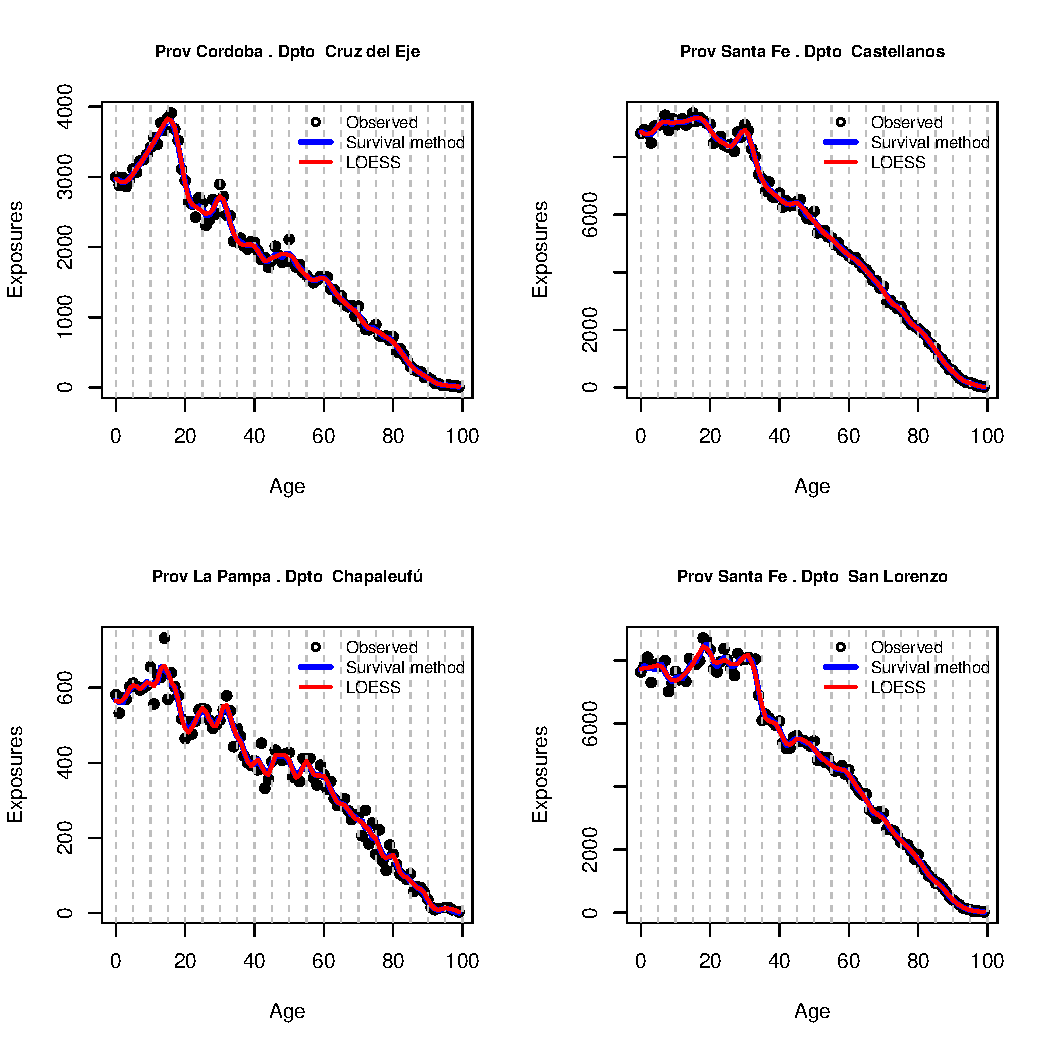
\includegraphics[width=0.7\linewidth]{analysis/plots/AdjExp} 

}

\caption{Ajuste de exposición 2008-2010. Cuatro casos. Fuente: elaboración propia en base a INDEC (2013)}\label{fig:AdjExp}
\end{figure}

\hypertarget{refs}{}
\leavevmode\hypertarget{ref-Camisa_2019}{}%
Camisa, Zulma C. 2019. ``Tabla Abreviada de Mortalidad de La Region
Pampeana de La Republica Argentina 1946-1948; Precedida de Un Analisis
Critico de Las Estadisticas Basicas.'' \emph{Repec.org}.
\url{https://econpapers.repec.org/paper/ecrcol048/8246.htm}.

\leavevmode\hypertarget{ref-FreireEtAl2015}{}%
Freire, Queiroz, F. H. M. d. A. 2015. ``Mortality Estimates and
Construction of Life Tables for Small Areas in Brazil, 2010.''

\leavevmode\hypertarget{ref-Gonzaga_Schmertmann_2016}{}%
Gonzaga, Marcos Roberto, and Carl Paul Schmertmann. 2016. ``Estimating
Age- and Sex-Specific Mortality Rates for Small Areas with Topals
Regression: An Application to Brazil in 2010.'' \emph{Revista Brasileira
de Estudos de População} 33 (3): 629--52.
\url{https://doi.org/10.20947/s0102-30982016c0009}.

\leavevmode\hypertarget{ref-Grushka2013}{}%
Grushka, Baum, C. 2013. ``Vivir Y Morir En Las Comunas de La Ciudad de
Buenos Aires: Un Estudio de Diferenciales.'' Población de Buenos Aires.

\leavevmode\hypertarget{ref-INDEC2015}{}%
INDEC. 2015. ``Estimaciones de Población Por Sexo, Departamento Y Año
Calendario2010-2025.''

\leavevmode\hypertarget{ref-James2014}{}%
James, Gareth, Daniela Witten, Trevor Hastie, and Robert Tibshirani.
2014. \emph{An Introduction to Statistical Learning: With Applications
in R}. Springer Publishing Company, Incorporated.

\leavevmode\hypertarget{ref-vanRaalte_Sasson_Martikainen_2018}{}%
Raalte, Alyson A. van, Isaac Sasson, and Pekka Martikainen. 2018. ``The
Case for Monitoring Life-Span Inequality.'' \emph{Science} 362 (6418):
1002--4. \url{https://doi.org/10.1126/science.aau5811}.

\leavevmode\hypertarget{ref-torcida2008}{}%
Torcida, Sebastián, Andrea L Vega, and Guillermo A Velázquez. 2008.
``Análisis de La Evolución de La Tasa de Mortalidad Infantil En Los
Departamentos de Argentina. 1994-20.''

\leavevmode\hypertarget{ref-Vaupel_Missov_2013}{}%
Vaupel, James W, and Trifon I Missov. 2013. ``Unobserved Population
Heterogeneity: A Review of Formal Relationships.'' \emph{Demographic
Research} 31. Demographic Research: 659--86.
\url{https://www.demographic-research.org/volumes/vol31/22/default.htm}.

\end{document}
